\documentclass{beamer}
\usetheme{Singapore}
\usepackage[utf8]{inputenc}
\usecolortheme{crane}
\usepackage{graphicx}
\usepackage{iwona}
\usepackage{standalone}
\usepackage{tikz}
\usetikzlibrary{arrows}
\usetikzlibrary{decorations.markings}
\usetikzlibrary{calc}
\usetikzlibrary{shapes,snakes}
\usepackage{amsmath}
\usepackage{amsfonts}
\usepackage{amsthm}
\usepackage{mathtools}


\beamertemplatenavigationsymbolsempty
\setbeamerfont{caption}{size=\tiny}


\title
{Queueing Networks for a Healthcare System}
\subtitle
{Deadlocking Properties}
\author{Geraint Palmer}
\date{Wales Mathematics Colloquium 2015 - Gregynog}


\begin{document}
\frame{\titlepage}

% THE PROBLEM - HEALTH BOARD, WORKFORCE PLANNING ETC

% 1st slide, health_system map
\begin{frame}
\frametitle{Aneurin Bevan University Health Board}
\begin{figure}
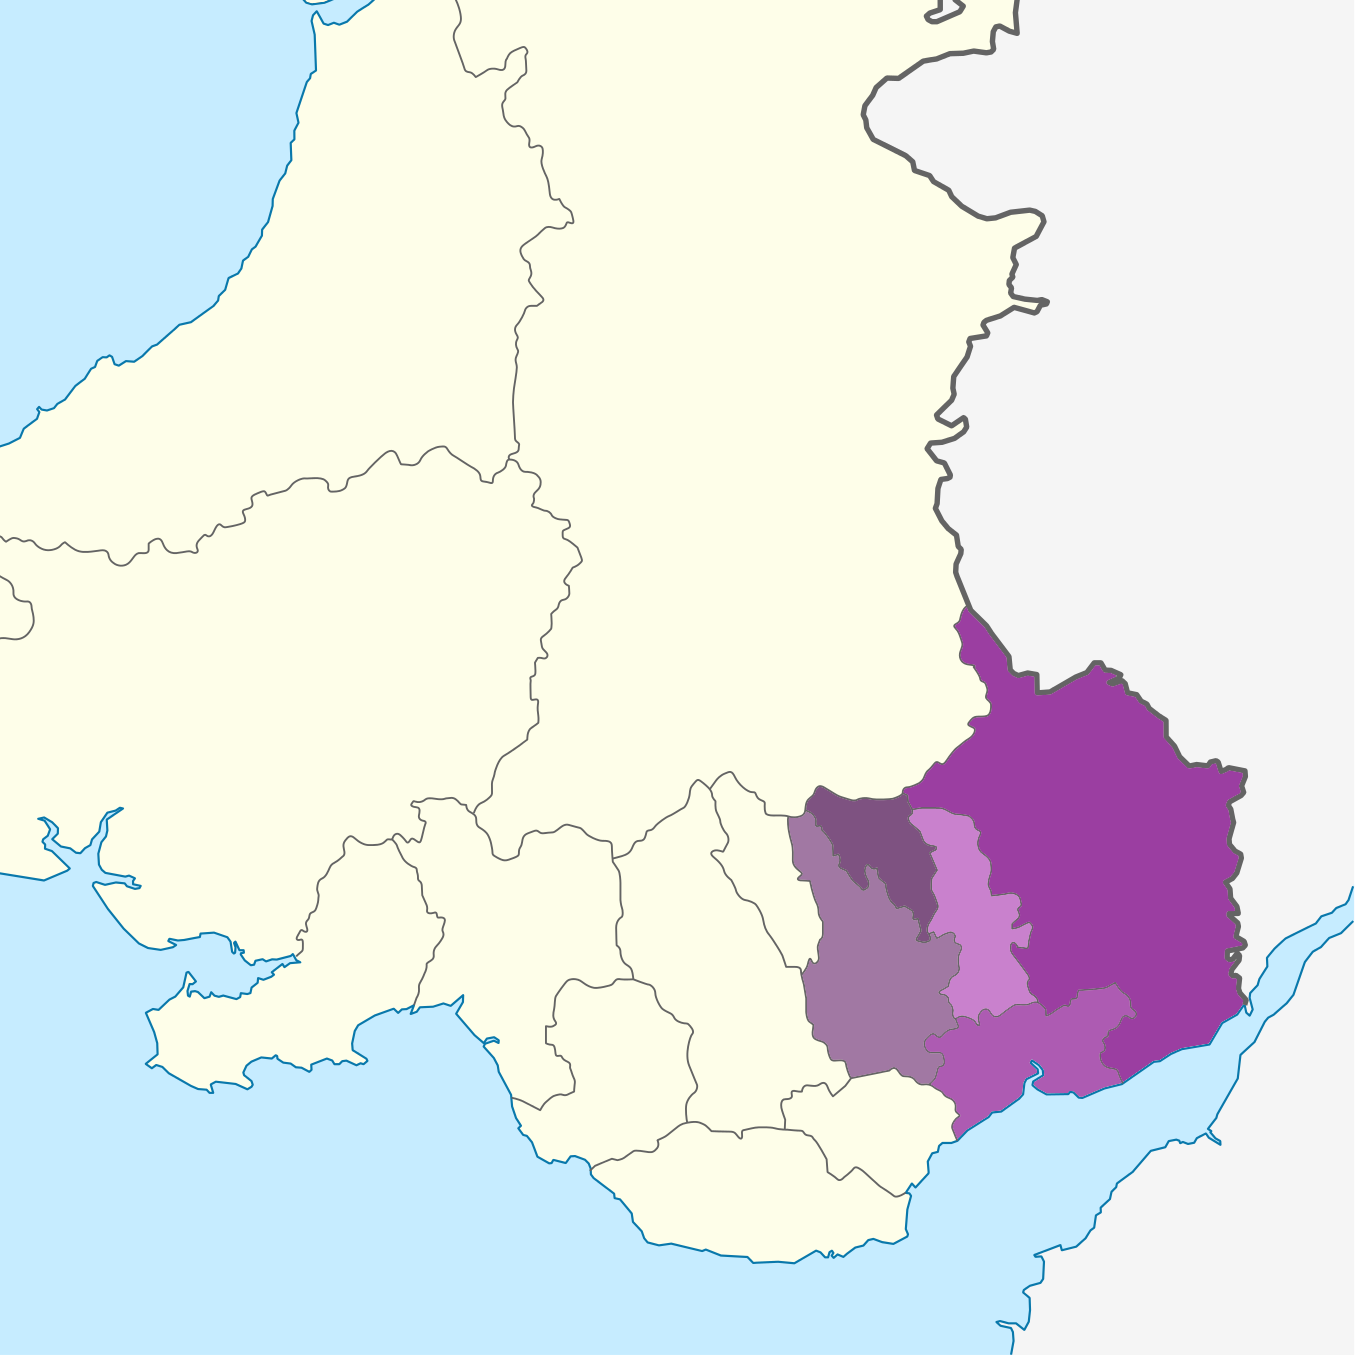
\includegraphics[width=0.7\textwidth]{Aneurin_Bevan}
\end{figure}
\end{frame}

% 1st slide, health_system map
\begin{frame}
\frametitle{Map of Healthcare System}
\begin{figure}
\includestandalone[width=\textwidth]{health_system}
\end{figure}
\end{frame}

% 3rd slide, example final product
\begin{frame}
    \includestandalone[width=\textwidth]{end_product}
\end{frame}

% 3rd slide, example final product
\begin{frame}
    \includestandalone[width=\textwidth]{end_product_results}
\end{frame}

\begin{frame}
    \frametitle{Deadlock}
    \begin{figure}
    \includestandalone[width=0.7\textwidth]{gridlock}
    \end{figure}
\end{frame}

\begin{frame}
    \begin{figure}
    \includestandalone[width=\textwidth]{buildupdigraph}
    \end{figure}
\end{frame}

% Markov deadlock model
\begin{frame}
    \frametitle{Markovian Model of Deadlock}
    \includestandalone[width=\textwidth]{2nodeexample}\newline
    \center{\LARGE{$(i, j)$}}
\end{frame}

\begin{frame}
%\frametitle{Markovian Model of Deadlock}
\center
\scriptsize \[S = \{(i,j)\in\mathbb{N}^{(n_1+2\times n_2+2)}| 0 \leq i + j \leq n_1 + n_2 + 2\}\cup\{(-1)\}\]
Define $\delta = (i_2, j_2) - (i_1, j_1)$\newline

  $q_{(i_1, j_1),(i_2, j_2)} = \left\{
  \begin{matrix*}[ r ]
    \left. \begin{matrix*}[ r ]
      \Lambda_1 & \text{if } i_1 \leq n_1 \\
      0 & \text{otherwise}
    \end{matrix*} \right\} & \text{if } \delta = (1, 0) \\
    \left. \begin{matrix*}[ r ]
      \Lambda_2 & \text{if } j_1 \leq n_2 \\
      0 & \text{otherwise}
    \end{matrix*} \right\} & \text{if } \delta = (0, 1) \\
    \left. \begin{matrix*}[ r ]
      (1 - r_{12})\mu_1 & \text{if } j_1 < n_1 + 2 \\
      0 & \text{otherwise}
    \end{matrix*} \right\} & \text{if } \delta = (-1, 0) \\
    \left. \begin{matrix*}[ r ]
      (1 - r_{21})\mu_2 & \text{if } i_1 < n_1 + 2 \\
      0 & \text{otherwise}
    \end{matrix*} \right\} & \text{if } \delta = (0, -1) \\
    \left. \begin{matrix*}[ r ]
      r_{12}\mu_1 & \text{if } j_1 < n_2 + 2 \\
      0 & \text{otherwise}
    \end{matrix*} \right\} & \text{if } \delta = (-1, 1) \\
    \left. \begin{matrix*}[ r ]
      r_{21}\mu_2 & \text{if } i_1 < n_1 + 2 \\
      0 & \text{otherwise}
    \end{matrix*} \right\} & \text{if } \delta = (1, -1) \\
    0 & \text{otherwise}
  \end{matrix*} \right.$\newline\newline

$q_{(i_1, j_1), (-1)} = \left\{
  \begin{matrix*}[ r ]
    r_{21}\mu_2 & \text{if } (i, j) = (n_1, n_2 + 2) \\
    r_{12}\mu_1 & \text{if } (i, j) = (n_1 + 2, n_2) \\
    0 & \text{otherwise}
  \end{matrix*}
  \right.$\newline\newline
$q_{-1, s} = 0$
\end{frame}

\begin{frame}
    \begin{figure}
    \includestandalone[width=0.95\textwidth]{markov_chain}
    \end{figure}
\end{frame}

\begin{frame}
    \frametitle{Times to Deadlock}
    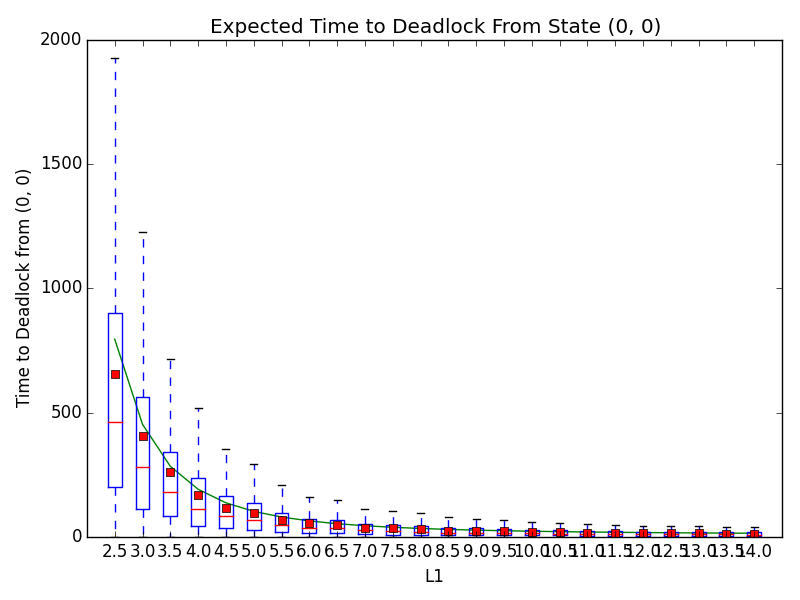
\includegraphics[width=0.5\textwidth]{varyL1}
    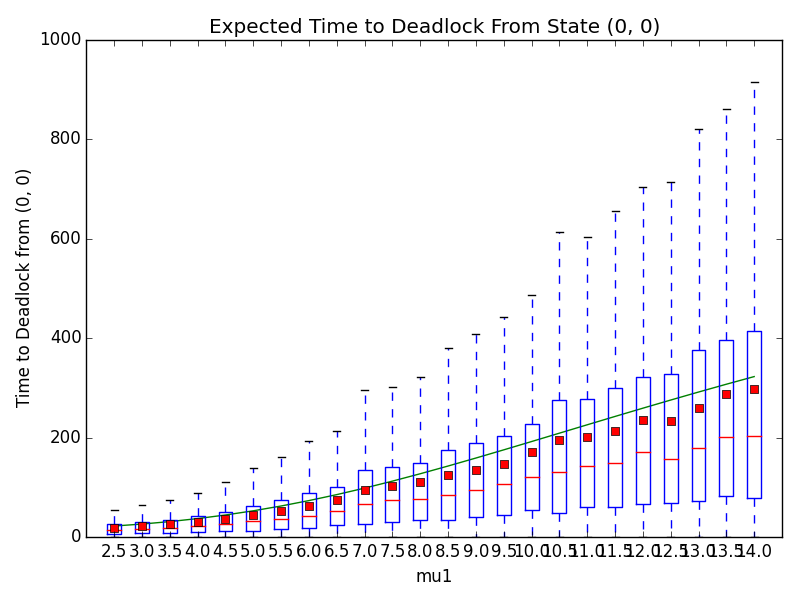
\includegraphics[width=0.5\textwidth]{varymu1}\newline
    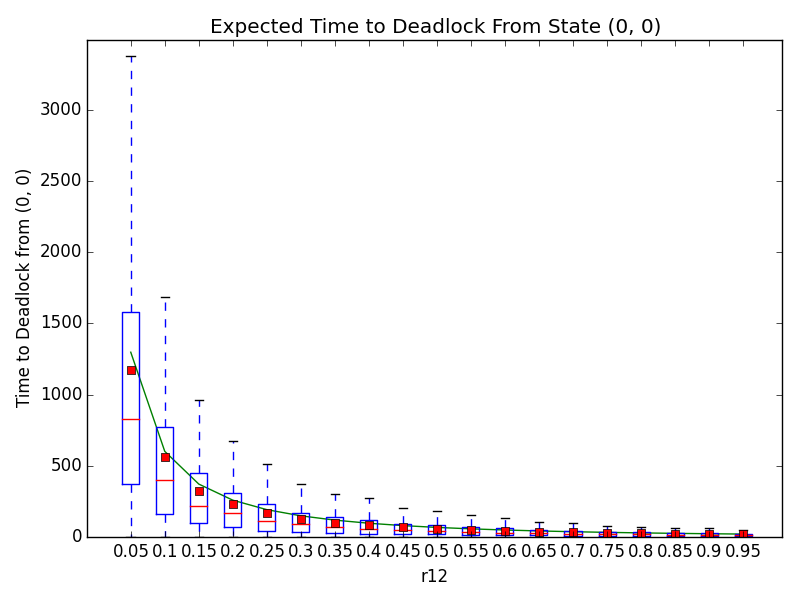
\includegraphics[width=0.5\textwidth]{varyr12}
    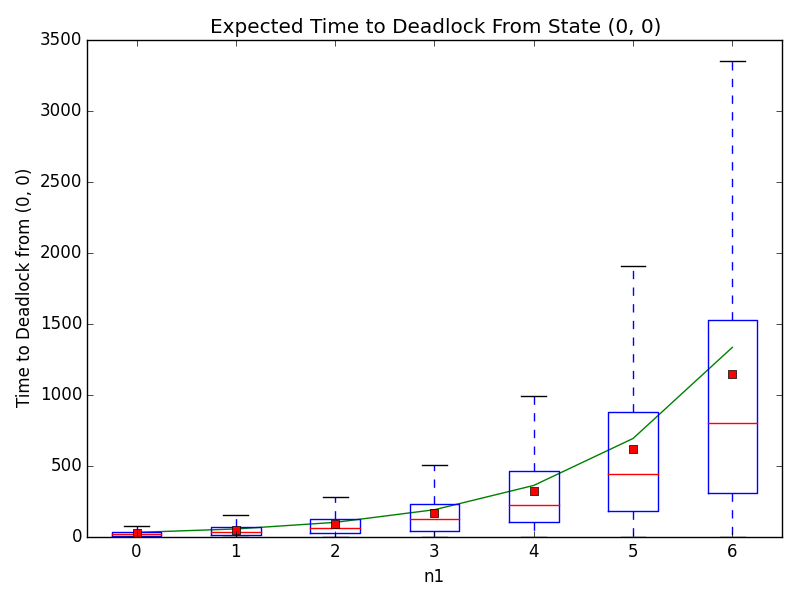
\includegraphics[width=0.5\textwidth]{varyn1}
\end{frame}

\begin{frame}
    \frametitle{Types of Deadlock}
    \begin{columns}
        \column{0.5\textwidth}
        \center
        Transient Deadlock
        \begin{figure}
        \includestandalone[width=\textwidth]{transientdeadlock}
        \end{figure}
        \column{0.5\textwidth}
        \center
        Absorbing Deadlock
        \begin{figure}
        \includestandalone[width=\textwidth]{absorbingdeadlock}
        \end{figure}
    \end{columns}
\end{frame}

\begin{frame}
    \frametitle{Future Work...}
    \begin{figure}
    \includestandalone[width=\textwidth]{future_work}
    \end{figure}
\end{frame}

% REINFORCEMENT LEARNING

\begin{frame}
    \frametitle{Reinforcement Leanrning}
    \only<1>{
    \begin{figure}
    \includestandalone[width=\textwidth]{health_system}
    \end{figure}
    }
    \only<2>{
    \begin{figure}
    \includestandalone[width=0.8\textwidth]{qlearn_flowchart}
    \end{figure}
    }
    \only<3>{
    Q-Learning
    \begin{equation*}
    Q(s, a) \leftarrow Q(s, a) + \alpha [ r + \gamma \text{max}_{a'} Q(s', a') - Q(s, a)]
    \end{equation*}
    }
\end{frame}

\begin{frame}
    \frametitle{Diolch - Thank You}
    https://github.com/geraintpalmer/Presentations
\end{frame}

\end{document}
